\documentclass{article}
\usepackage[preprint]{neurips_2026}
\usepackage[T1]{fontenc}
\usepackage[utf8]{inputenc}
\usepackage{microtype}
\usepackage{amsmath,amssymb,booktabs,array,multirow}
\usepackage{graphicx}
\usepackage{hyperref}
\hypersetup{pdftitle={Resutura: Effect-Semantic Recovery for Computer-Use Agents},pdfauthor={Aura Yavary},pdfsubject={NeurIPS 2026-style preprint},colorlinks=true,linkcolor=black,citecolor=black,urlcolor=blue}
\usepackage{xcolor}
\usepackage{tikz}
\usetikzlibrary{arrows.meta,positioning,fit}

\title{Resutura: Effect-Semantic Recovery for Computer-Use Agents}

\author{%
Aura Yavary\\
University of California, Davis
}

\begin{document}
\maketitle

\begin{abstract}
Computer-use agents can recover from a failed local action while still leaving the external world in the wrong state. A lost acknowledgement may hide a successful commit; a misdirected write may require a compensating action; another actor may concurrently make a valid change that recovery must preserve; and an irreversible bad effect may admit no safe automated repair. Existing work already studies causal repair, checkpoint rewind, compensation, transactional tool runtimes, verify-before-retry, exactly-once execution, and harm recovery. We therefore study a narrower systems question: \emph{can one recovery runtime select the appropriate recovery semantics after divergence---verify and continue, rewind, compensate, preserve concurrent state, or stop---while retaining valid task progress?} Resutura separates checkpointed local state from externally committed effects, records effect ownership and declared tool capabilities, and emits auditable recovery certificates. In a deterministic diagnostic suite, Resutura distinguishes compensable misdirection, ambiguous commit, concurrent valid state, and non-compensatable effects; a tool-contract matrix shows that readback or idempotency can make simpler baselines sufficient. Component ablations isolate the roles of compensation, contract awareness, and effect ownership. A headless-Chromium mechanism-transfer tier confirms the same qualitative behaviors outside a pure Python state simulator while keeping the action policy deterministic. The reported results validate recovery semantics and research infrastructure only; we do not claim frontier-model or state-of-the-art computer-use performance.
\end{abstract}

\section{Introduction}
Long-horizon computer-use agents increasingly act through interfaces whose consequences do not share one rollback domain. A local checkpoint may restore a browser tab, a document buffer, or an agent context while a remote message, publication, payment, or durable record remains committed. The failure signal seen by the agent is therefore insufficient to determine the correct recovery action. A timeout may mean ``nothing happened'' or ``the write happened but the acknowledgement was lost.'' Replaying the same action can either complete required work or duplicate a consequential effect.

This paper studies \emph{effect-semantic recovery}: choosing recovery behavior based on the realized external state and the guarantees exposed by the tool contract. We focus on the decision boundary after a computer-use trajectory has diverged, rather than on improving the underlying model's planning ability. The central question is:

\begin{quote}
\emph{Can a computer-use recovery runtime choose when to verify, locally repair, rewind, compensate, preserve unrelated valid state, or stop?}
\end{quote}

Resutura implements this decision contract and packages it with falsifiable diagnostic suites. The system tracks a joint state consisting of local/rewindable state and externally committed effects; records effect ownership; treats concurrent valid changes as protected invariants; and refuses to fabricate success when no safe compensator exists. Figure~\ref{fig:overview} summarizes the loop.

Our contributions are deliberately narrow:
\begin{itemize}
    \item an executable effect-semantic recovery contract for computer-use workflows;
    \item a diagnostic suite in which the correct response changes qualitatively across effect classes;
    \item a tool-contract factorization showing when readback or idempotency makes simpler recovery policies sufficient;
    \item component ablations and evidence artifacts that connect claims to deterministic raw traces;
    \item a real Chromium mechanism-transfer tier plus a provider-neutral policy boundary, without overstating these as frontier-model evidence.
\end{itemize}

\begin{figure}[t]
\centering
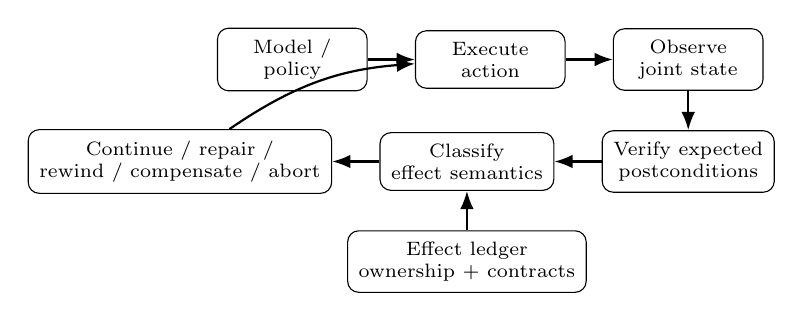
\begin{tikzpicture}[font=\scriptsize, node distance=5mm and 6mm,
box/.style={draw,rounded corners,align=center,inner sep=4pt,minimum width=19mm},
arr/.style={-Latex,thick}]
\node[box] (policy) {Model /\\policy};
\node[box,right=of policy] (act) {Execute\\action};
\node[box,right=of act] (observe) {Observe\\joint state};
\node[box,below=of observe] (verify) {Verify expected\\postconditions};
\node[box,left=of verify] (class) {Classify\\effect semantics};
\node[box,left=of class,minimum width=26mm] (recover) {Continue / repair /\\rewind / compensate / abort};
\node[box,below=of class,minimum width=27mm] (ledger) {Effect ledger\\ownership + contracts};
\draw[arr] (policy)--(act);
\draw[arr] (act)--(observe);
\draw[arr] (observe)--(verify);
\draw[arr] (verify)--(class);
\draw[arr] (class)--(recover);
\draw[arr] (ledger)--(class);
\draw[arr,bend left=15] (recover) to (act);
\end{tikzpicture}
\caption{Resutura separates action policy from recovery semantics. Online recovery uses observable state and declared tool capabilities; forked counterfactual replay is reserved for offline analysis and is not used as an oracle for policy selection.}
\label{fig:overview}
\end{figure}

\section{Related work and positioning}
The surrounding area is already rich. CausalFlow converts failed traces into minimal counterfactual repairs~\cite{causalflow}; CUADebug localizes root causes in failed computer-use trajectories and guides corrective re-execution~\cite{cuadebug}; AgentRewind and Rollback-Induced Reflection study recovery around checkpoints and rollback boundaries~\cite{agentrewind,rir}. Robust Agent Compensation, Atomix, and Cordon develop compensation and transaction-like tool execution semantics~\cite{rac,atomix,cordon}. ACRFence studies irreversible effects across checkpoint restore~\cite{acrfence}. Verification-aware wrappers use postcondition checks and verify-before-retry under non-atomic failures~\cite{verified}. Revisable by Design formalizes idempotent, reversible, compensable, and irreversible action classes~\cite{revisable}. Recent exactly-once work shows that model behavior, harness behavior, and tool contracts jointly determine duplicate effects~\cite{limbo}. Safety-invariant work targets irreversible transitions~\cite{safetyinvariants}, while Human-Guided Harm Recovery studies preference-aligned post-harm recovery for computer-use agents~\cite{harmrecovery}. CONTINUITY addresses consequence integrity across composed security controls~\cite{continuity}, and StateAct uses program-state grounding plus independent completion verification in long-horizon computer use~\cite{stateact}.

Resutura therefore does \emph{not} claim to invent rollback, compensation, idempotency, causal repair, effect ledgers, or reversibility taxonomies. Its contribution hypothesis is narrower: an integrated CUA recovery decision contract and evaluation suite in which different realized effect states demand different recovery semantics.

\section{Effect-semantic recovery}
\subsection{Joint state and effect contracts}
Let the joint state be $s=(s^L,s^E)$, where $s^L$ is local/rewindable state and $s^E$ is externally committed state. A consequential action $a_t$ may declare expected postconditions $P_t$, an intended target, and a tool contract $K_t$ containing capabilities such as authoritative readback, idempotency, or a compensator. The runtime maintains an effect ledger $E$ with ownership, commit status, and compensation status.

A checkpoint restores $s^L$ but does not silently erase $s^E$. This distinction is critical: restoring the agent's execution is not equivalent to restoring the world.

\subsection{Recovery classes}
After a divergence, Resutura distinguishes five classes.

\paragraph{Verified commit.} The call result is ambiguous, but authoritative postconditions show that the intended effect committed. Continue without replay.

\paragraph{Compensable wrong effect.} An agent-owned wrong effect committed and a valid compensator exists. Apply forward compensation and then the intended action.

\paragraph{Concurrent valid state.} External state that is not owned by the failed action is treated as a protected invariant and must survive recovery.

\paragraph{Non-compensatable effect.} The bad effect cannot be safely undone. Stop and escalate rather than report fabricated task success.

\paragraph{Local reversible failure.} When no external commitment prevents rollback, local repair, subgoal reconstruction, or rewind remains admissible.

Candidate recovery $r$ can be analyzed by
\begin{equation}
U(r)=P(\mathrm{recover}\mid r)-\lambda_c C(r)-\lambda_l L(r)-\lambda_s R(r)-\lambda_p\Delta_{\mathrm{progress}}(r)-\lambda_d D_{\mathrm{collateral}}(r),
\end{equation}
subject to task postconditions and protected invariants. The bundled online controller does not use simulator-only forked outcomes to select $r$. Counterfactual forks are retained only for offline diagnostics.

\subsection{Recovery certificate}
Each recovery emits a certificate containing the diagnosed state slice, considered alternatives, verified postconditions, protected invariants, progress-preservation result, external-effect reconciliation status, and safe-abort status. This makes recovery behavior inspectable at the level of world-state consequences rather than only final task completion.

\section{Experimental setup}
\subsection{Workflow and baselines}
The deterministic workflow gathers research facts, populates a spreadsheet, writes a comparison document, saves artifacts, and publishes the result. The environment exposes local application state and a separate external-effect ledger. We compare five scaffolds:

\textbf{Base} executes the workflow without recovery; \textbf{Retry} blindly retries one failed action; \textbf{Verify} uses authoritative postcondition readback before retry; \textbf{Rewind} restores a checkpointed local state; and \textbf{Resutura} selects effect-semantic recovery.

Unless otherwise noted, deterministic simulator cells contain 40 paired trials per method/scenario. We report task success as well as effect-level outcomes such as duplicate effects, unreconciled wrong effects, protected-state loss, and safe abort. The release contains deterministic seeds, raw trajectories, experiment registries, and claim-to-evidence hashes.

\subsection{Effect Semantics Suite}
Table~\ref{tab:effects} evaluates four effect classes.

\begin{table}[t]
\centering
\small
\begin{tabular}{lccccc}
\toprule
Scenario & Base & Retry & Verify & Rewind & Resutura \\
\midrule
Compensable misdirection & 0 & 0 & 0 & 0 & \textbf{100} \\
Ambiguous commit & \textbf{100} & 0 & \textbf{100} & 0 & \textbf{100} \\
Concurrent valid + misdirection & 0 & 0 & 0 & 0 & \textbf{100} \\
Non-compensatable misdirection & 0 & 0 & 0 & 0 & 0$^{\dagger}$ \\
\bottomrule
\end{tabular}
\caption{Task success (\%) in the deterministic Effect Semantics Suite. $^{\dagger}$Resutura safe-aborts in 100\% of non-compensatable trials; zero task success is intentional.}
\label{tab:effects}
\end{table}

\paragraph{Compensable misdirection.} The final publication commits to the wrong target. Base, Retry, Verify, and Rewind leave the wrong external effect unreconciled. Resutura retracts only the agent-owned wrong effect and publishes to the intended target.

\paragraph{Ambiguous commit.} The intended publication commits, but the acknowledgement is lost. Base succeeds by doing nothing. Retry and Rewind duplicate the intended effect under a non-idempotent contract. Verify and Resutura both use authoritative readback and continue without replay; this tie is expected and important.

\paragraph{Concurrent valid change.} Another actor creates a valid external update before the agent's misdirected publication. Recovery must compensate the agent-owned error without deleting the unrelated update. Effect ownership is therefore a correctness condition, not only an accounting convenience.

\paragraph{Non-compensatable effect.} The wrong effect commits with no safe compensator. Resutura reports failure and safe-aborts rather than optimizing the task metric at the expense of correctness.

\subsection{Component ablations}
Table~\ref{tab:ablations} removes one mechanism at a time. Removing compensation destroys recovery on wrong-target effects. Ignoring tool-contract evidence turns ambiguous commits into blind replay and duplicate effects. Removing effect ownership preserves simple misdirection recovery but fails when a concurrent valid update must be protected.

\begin{table}[t]
\centering
\small
\begin{tabular}{lcccc}
\toprule
Variant & Misdirect & Ambiguous & Concurrent & Non-comp. \\
\midrule
Full Resutura & 100 & 100 & 100 & 100 abort \\
$-$ compensation & 0 & 100 & 0 & 100 abort \\
$-$ contract awareness & 100 & 0 & 100 & 100 abort \\
$-$ effect ownership & 100 & 100 & 0 & 100 abort \\
\bottomrule
\end{tabular}
\caption{Deterministic component ablations (40 paired trials per cell). Values are task success percentages except the final column, which reports safe-abort rate.}
\label{tab:ablations}
\end{table}

\section{Tool-contract factorization}
The Effect Semantics Suite uses authoritative readback without tool-level idempotency. To expose dependence on the tool rather than the runtime, we add an \emph{unobservable ambiguous commit}: a write commits but the failed call result contains no evidence of the commit. We then factor authoritative readback and idempotency (Table~\ref{tab:contracts}).

\begin{table}[t]
\centering
\small
\begin{tabular}{lccccc}
\toprule
Contract & Base & Retry & Verify & Rewind & Resutura \\
\midrule
Readback only & 100 & 0 & 100 & 0 & 100 \\
Idempotency only & 100 & 100 & 100 & 100 & 100 \\
Readback + idempotency & 100 & 100 & 100 & 100 & 100 \\
Neither & 100$^*$ & 0 & 0$^{\ddagger}$ & 0 & 0$^{\ddagger}$ \\
\bottomrule
\end{tabular}
\caption{Task success (\%) under an unobservable ambiguous commit. $^*$Base leaves the world correct because it does not replay but has no evidence of success. $^{\ddagger}$Verify and Resutura safe-abort in 100\% of trials.}
\label{tab:contracts}
\end{table}

The matrix deliberately removes a universal ``Resutura wins'' narrative. Readback is sufficient for the verification-aware baseline to match Resutura on this fault. Tool-level idempotency is sufficient for Retry and Rewind to avoid duplicates. With neither capability, a runtime cannot generally infer whether replay is safe from the failed acknowledgement alone; conservative abort avoids duplication but sacrifices known completion. This result is consistent with recent evidence that exactly-once behavior depends strongly on tool contracts~\cite{verified,limbo}.

The study also exposed a simulator bug: checkpoint restore originally rewound the server-side idempotency registry. That behavior was incorrect because deduplication state belongs to the external rollback domain. The registry now survives local rewind.

\section{Chromium mechanism transfer and policy boundary}
The release exposes a provider-neutral policy interface. A policy receives task context, the current observation, declared tool capabilities, and recent history, and returns an action plus expected postconditions. Resutura independently executes, verifies, classifies divergence, and selects recovery semantics. A recorded-policy experiment validates this boundary but is explicitly not model evidence.

We additionally port the workflow to a real headless Chromium DOM. In a paired mechanism-transfer diagnostic (two deterministic trials per method/scenario), the qualitative simulator findings survive: Resutura reconciles wrong-target committed effects, preserves a concurrent valid publication while compensating its own misdirection, safe-aborts on a non-compensatable committed effect, and matches verification-aware recovery on ambiguous commit. This tier shows that the mechanism is not solely an artifact of Python dictionaries. Because the action policy is deterministic and external effects remain harness-controlled, it does not establish frontier-model computer-use performance.

\section{Evidence quality and unexpected findings}
The project maintains an evidence layer containing experiment logs, failed experiments, decision logs, raw trajectories, qualitative cases, and a claim-to-evidence map. Several findings are intentionally awkward rather than promotional.

First, Base achieves 100\% task success on ambiguous commit by simply not retrying; task success alone therefore cannot distinguish correct recovery from lucky inaction. Second, verification-aware recovery ties Resutura whenever readback completely resolves the fault. Third, idempotency can make blind Retry and Rewind sufficient. Fourth, non-compensatable effects are a case in which a correct recovery policy should fail the task and escalate. Finally, stress testing found benchmark bugs---including stateful perturbations accidentally reused across methods and a grader that initially treated valid concurrent state as damage. These bugs were retained in the experiment journal rather than erased from the development narrative.

\section{Dataset and uncertainty}
The release packages 160 public scenario/task records and 800 raw method trajectories as JSONL/GZIP, together with a schema, split manifest, and source-run hash. Public dev/test labels are for analysis hygiene only and are not hidden evaluation data. For the deterministic simulator we report Wilson 95\% binomial intervals and paired-seed contrasts as descriptive diagnostics. These intervals must not be interpreted as uncertainty over frontier-model behavior. The Chromium tier has only two paired trials per method/scenario and is intentionally excluded from statistical or state-of-the-art claims.

\section{Limitations and falsification criteria}\label{sec:limitations}
The primary environment is deterministic; the Chromium tier exercises real DOM state while keeping the planner deterministic. Effect contracts and compensators are explicit. The failure localizer is rule-based. No frontier model drives the reported actions, and consequential external services remain harness-controlled. The experiments establish that the recovery semantics are implemented and behaviorally distinguishable, not that a model can infer them in open-world computer use.

A stronger study should factor \textbf{model $\times$ harness $\times$ tool contract} in side-effect-capable browser or desktop tasks, including lost acknowledgements, delayed visibility, redelivery, compensable and non-compensatable writes, concurrent legitimate changes, and authorization boundaries. The Resutura hypothesis should be considered unsupported if a verification-aware baseline matches it across the broader effect classes, if transactional staging dominates without sacrificing completion, if the effect classifier requires privileged labels unavailable to real agents, or if safe abort is poorly calibrated.

\section{Conclusion}
A failed tool result does not uniquely determine a recovery action. Depending on realized effect state and available tool guarantees, the correct response may be to continue, verify, rewind, compensate, preserve concurrent state, or stop. Resutura turns that distinction into an executable computer-use recovery contract and a falsifiable diagnostic suite. The remaining empirical question is whether this contract improves reliability when effect semantics must be inferred under real model-driven computer-use uncertainty.

\begin{thebibliography}{16}
\bibitem{causalflow} A. Bonagiri, D. Borkar, G. J. Anderias, S. Rafatirad, and H. Homayoun. \emph{CausalFlow: Causal Attribution and Counterfactual Repair for LLM Agent Failures}. arXiv:2605.25338, 2026.
\bibitem{cuadebug} W. Zhang et al. \emph{CUADebug: Diagnosing and Repairing Computer-Use Agent Failures}. arXiv:2608.02643, 2026.
\bibitem{agentrewind} Y. Zhuang et al. \emph{AgentRewind: Recoverable Execution for Long-Horizon LLM Agents}. arXiv:2608.14380, 2026.
\bibitem{rir} Y. Yu, L. Yao, Y. Li, E. Wang, and L. Wu. \emph{Rollback the World, Keep the Reflection: Rollback-Induced Reflection for Long-Horizon LLM Agents}. arXiv:2609.18304, 2026.
\bibitem{rac} S. Perera, K. Hapuarachchi, F. Leymann, and R. Khalaf. \emph{Robust Agent Compensation (RAC): Teaching AI Agents to Compensate}. arXiv:2605.03409, 2026.
\bibitem{atomix} B. Mohammadi et al. \emph{Atomix: Timely, Transactional Tool Use for Reliable Agentic Workflows}. arXiv:2602.14849, 2026.
\bibitem{cordon} Z. Chen et al. \emph{Cordon: Semantic Transactions for Tool-Using LLM Agents}. arXiv:2606.17573, 2026.
\bibitem{acrfence} Y. Zheng, Y. Yang, W. Zhang, and A. Quinn. \emph{ACRFence: Preventing Semantic Rollback Attacks in Agent Checkpoint-Restore}. arXiv:2603.20625, 2026.
\bibitem{verified} I. K. Mansoor, A. Phadke, and P. Rana. \emph{Verified Tool Calls Improve LLM Agent Reliability Under Non-Atomic Failures}. arXiv:2608.02645, 2026.
\bibitem{revisable} Z. Zhai, M. Li, and X. Wang. \emph{Revisable by Design: A Theory of Streaming LLM Agent Execution}. arXiv:2604.23283, 2026.
\bibitem{limbo} J. Li. \emph{Where Does Exactly-Once Live? Model, Harness, and Tool-Contract Effects on Duplicate Side Effects in LLM Agents}. arXiv:2609.29095, 2026.
\bibitem{safetyinvariants} Z. Yin. \emph{Safety Invariants for Agents Orchestrating Irreversible State Transitions: A Four-Dimensional Formalism Evaluated on Public Ledgers}. arXiv:2608.00783, 2026.
\bibitem{harmrecovery} C. Li, S. CH-Wang, A. Peng, and A. Bobu. \emph{Human-Guided Harm Recovery for Computer Use Agents}. arXiv:2604.18847, 2026.
\bibitem{continuity} C. Zheng and G. Yang. \emph{CONTINUITY: Security-Context Contracts for Composable LLM Agent Controls}. arXiv:2609.05269, 2026.
\bibitem{stateact} Y. Yang et al. \emph{StateAct: Program State, before Pixels, for Long-Horizon Computer-Use Agents}. arXiv:2607.22798, 2026.
\end{thebibliography}

\section*{NeurIPS Paper Checklist}
\small
\begin{enumerate}
\item \textbf{Claims.} \textbf{Yes.} The abstract, experiments, and limitations distinguish deterministic mechanism evidence, Chromium mechanism-transfer evidence, and unmeasured model-backed performance.
\item \textbf{Limitations.} \textbf{Yes.} Limitations are stated explicitly in Section~\ref{sec:limitations}.
\item \textbf{Theory assumptions and proofs.} \textbf{N/A.} The paper introduces an executable recovery contract rather than a new theorem.
\item \textbf{Experimental reproducibility.} \textbf{Yes.} The release includes deterministic seeds, manifests, raw traces, experiment registries, and one-command audits.
\item \textbf{Open access to data and code.} \textbf{Yes, in the accompanying research release.} Public repository hosting may be added separately; no unavailable URL is fabricated in this preprint.
\item \textbf{Experimental settings and details.} \textbf{Yes.} The paper reports scenario definitions, baselines, trial counts, contract capabilities, and evidence tiers.
\item \textbf{Statistical significance.} \textbf{Yes, with scope limits.} Wilson intervals and paired-seed contrasts are descriptive for the deterministic simulator and are not presented as model uncertainty.
\item \textbf{Compute resources.} \textbf{Yes.} The bundled studies use CPU execution and headless Chromium; no model training or GPU cluster is required for the reported results.
\item \textbf{Code of ethics.} \textbf{Yes.} The experiments use synthetic/harness-controlled environments and do not involve human subjects or real consequential services.
\item \textbf{Broader impacts and misuse.} \textbf{Yes.} The work concerns recovery from consequential tool effects; unsafe automation and over-trusting compensators are discussed in limitations.
\item \textbf{Safeguards.} \textbf{Yes.} Non-compensatable effects trigger safe abort rather than fabricated success.
\item \textbf{Licenses for existing assets.} \textbf{Yes where applicable.} The release records its own license and references public research artifacts by citation rather than redistributing them.
\item \textbf{New assets documentation.} \textbf{Yes.} Dataset cards, benchmark cards, schemas, evidence maps, and reproduction matrices are included in the release.
\item \textbf{Human subjects / crowdsourcing.} \textbf{N/A.} No human-subject study or crowdsourced labeling was performed.
\item \textbf{Institutional review.} \textbf{N/A.} No human participants or sensitive personal data are involved.
\item \textbf{Use of generative AI in manuscript preparation.} The author is responsible for the scientific content, citations, claims, and final text. AI-assisted drafting/editing must be reviewed and verified by the author before public submission.
\end{enumerate}
\normalsize


\end{document}
